\section{Technique}
\label{sec:technique}

In this section, we formalize our technique for reasoning about movement within a coarse `unit cube' space.
Starting from spatial traces, we map sequences of positions into both occupied cubes as well as nodes in a graph, then discuss three classes of properties: individual actor properties, multiple actor properties, and properties of paths.

\subsection{Foundations and Definitions}
We begin with a time-sequenced trace $T$ of spatial data, $T = (t,x,y,z)$ where $t$ is a time referenced to some global start time, and $x,y,z$ are real numbers $\in \mathbb{R}$. 
Let trace T be indexed by $i$ so that $T_i$ is the $i$th time-ordered record in $T$.

We call the thing that is moving an \eb{actor}, designated by $\bigstar$.

Let there exist a space $C^3 \equiv \mathbb{Z}^3$ called ``cube 3".
We denote two functions: $f_{cube}$ for mapping from a trace record $T_i$ and $f_{node}$ that maps from $T_i$ to a node in a graph $G$. The symbol $\alpha$ scales positions from the original unit of measure to the size of the unit cube (See Sect~\ref{sec:tool} for discussion of choosing the size of the unit cube).

$$f_{cube}(T_i = (t,x,y,z)) = (\lfloor \alpha * x \rfloor, \lfloor \alpha * y \rfloor , \lfloor \alpha * z \rfloor ) = cube_i$$

$$f_{node}(t,x,y,z) = v_i | V = V \cup v_i$$


A spatial abstraction $\cube$ is a tuple $(\mathbb{T}, G, R, C^3, F, A)$, where $\mathbb{T}$ is a set of traces, $G$ is a directed multigraph, $R$ is a relation mapping $cube_i$ to graph node $v_i$, $C^3$ is the unit cube space, $F$ is the successor relation mapping edges in $G$ to their successors, and $A$ is a relation mapping actor $\bigstar_i$ to trace $T$.


%Let the $i$th element of the trace file be designated $\T_i$, and to the position data in $\bigstar_i$ we apply $f_{\cube}$ and infer the existence of cube $\cube_i$.

%$$\bigstar_i \Rightarrow (\cube_i | \cube_{xyz\in \mathbb{N}} = f_{\cube}(\bigstar_{xyz})$$ 

This maps every record in the trace file to a cube.
Simultaneously, we create a root node $v_i$ in a directed multigraph $G = (V,E)$.
For each subsequence trace record $\bigstar_{i+1}$, we check if this position maps to the same cube, $\cube_i$, or to a new cube, $\cube_{j}.$
If a record maps to a new cube $\cube_{j}$, then we add a directed edge to $E$ from $v_i$ to $v_{j}$.  
We add a label the edge $(v_i, v_j)$ with the time $t$.
The node $v_i$ corresponds to $\cube_i$ and the node $v_{j}$ corresponds to $\cube_{j}$.
From the existence of this edge we say there is a path from $\cube_i$ to $\cube_j$ denoted $\cube_{i\rightsquigarrow j}$.  More formally,

$$ f_{\cube}(\bigstar_i) \neq f_{\cube}(\bigstar_{i+1}) \Rightarrow (v_i, v_j) \in E \equiv \cube_{i\rightsquigarrow j} $$


Now we have a way to map a sequence of positions records to a unit cube space in which we have embedded a graph.
The edges in the graph capture the timestamp for each position.
We are now ready to begin reasoning about properties.


\subsection{Properties of Single Actors}

\emph{Note: all properties in this table a limited to a particular actor $\bigstar_i$.}
\begin{tabular}{| p{2.8cm} | p{11.5cm} | }
\hline
PROPERTY & FORMALISM \\ \hline
% Move to multiple places & $\phi_{\{multiplePlaces\}} = \exists (P(b_{home}, b_a), P(b_{home}, b_b)| b_a \neq b_a)$ \\ \hline
Move to multiple places & $\phi_{\{multiplePlaces\}} = |V| > 1$ \\ \hline
Returns Home & $\phi_{\{returnhome\}} = \exists P(b_{home}, b_{home})$ \\ \hline
No repetition & $\phi_{\{noRepetition\}} = \forall e(v_a, v_b), e(v_c,v_d) in E, v_b \neq v_c, v_a \neq v_d$ \\ \hline
 Loiters & $\phi_{\{loiters\}} =  \exists e \in E$ such that $e[time] - e_{prev}[time] > k$, where $k$ is time bound \\ \hline
 & \\ \hline
 & \\ \hline
$\phi_{\{teleport\}}$ & $  \exists  p_t, p_{t+1} | \lnot Adjacent(b_{p_t}, b_{p_{t+1}})$ \\ \hline
Hot Box & $\phi_{\{hotBoxOfSizeN\}} = \exists b_i, v_i \in E | n \geq |\{e \in E | e(v_x, v_i), v_x \in E\}$ \\ \hline
\end{tabular}


\subsection{Properties of Multiple Actors}
\begin{tabular}{| p{2.8cm} | p{11.5cm} | }
\hline
PROPERTY & FORMALISM \\ \hline
 Crumb independence (given graphs of $n$ actors)& $\phi_{\{crumbInd\}} =  i,j \in \{1..n\} \land i \neq j \rightarrow V_i \cap V_j = \emptyset $ \\ \hline
 Following crumbs & $\phi_{\{following\}} =  \exists E' \subset E_1 \land E'' \subset E_2$ such that $path(E')=path(E'') $  \\ \hline
% not sure how to do these formulas in a nice way with graphs yet
% these are only for two entities
 Above & $T_1[i].z > T_2[i].z \forall i$ where $i$ is indexing a time interval\\ \hline
 Below & $T_1[i].z < T_2[i].z \forall i$ where $i$ is indexing a time interval\\ \hline
 Front & $T_1[i].x > T_2[i].x \forall i$ where $i$ is indexing a time interval\\ \hline
 Behind & $T_1[i].x < T_2[i].x \forall i$ where $i$ is indexing a time interval\\ \hline
 Right & $T_1[i].y < T_2[i].y \forall i$ where $i$ is indexing a time interval \\ \hline
 Left & $T_1[i].z < T_2[i].z \forall i$ where $i$ is indexing a time interval \\ \hline
\end{tabular}


\subsection{Properties of Paths}
\subsubsection{The Ratio Cube}

\begin{wrapfigure}{l}{0.3\textwidth}
  \centering
    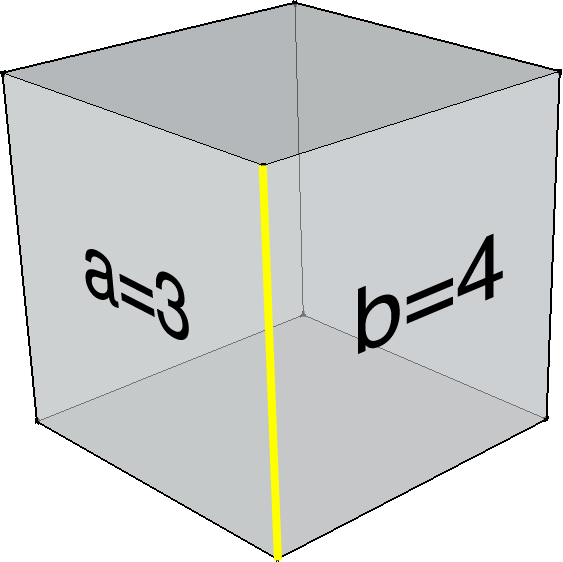
\includegraphics[width=0.3\textwidth]{./figures/ratioCube_3_4}
      \caption{The ratio cube.}
      \label{fig:ratioCube}
\end{wrapfigure}
In order to compare multiple path, we consider for each path $P$ a method of counting how many times an actor moves in each direction.  
In our model, there are six directions: up, down, left, right, forward, back, and we assign a counter to each.
We then compare the ratios of the counters, and use this ratio as a way of comparing multiple paths.
A visual representation of these counters and the ratio between faces is shown in Fig.~\ref{fig:ratioCube}.
As shown in the figure, the number of moves in each direction is associated with a face of the ratio cube, and the ratios between the directions is associated with the edges of the cube.


Figures~\ref{fig:3by4}-\ref{fig:6by8_squiggle} show ratio equivalent paths, that is, the ratio of the number of moves made in each of the size directions is the same.
These ratios are invariant under transformation by scale, and two paths that make the same ratio of moves in any order are likewise equivalent.


\begin{figure}
\centering
  \begin{minipage}[t]{.45\textwidth}
  \centering
  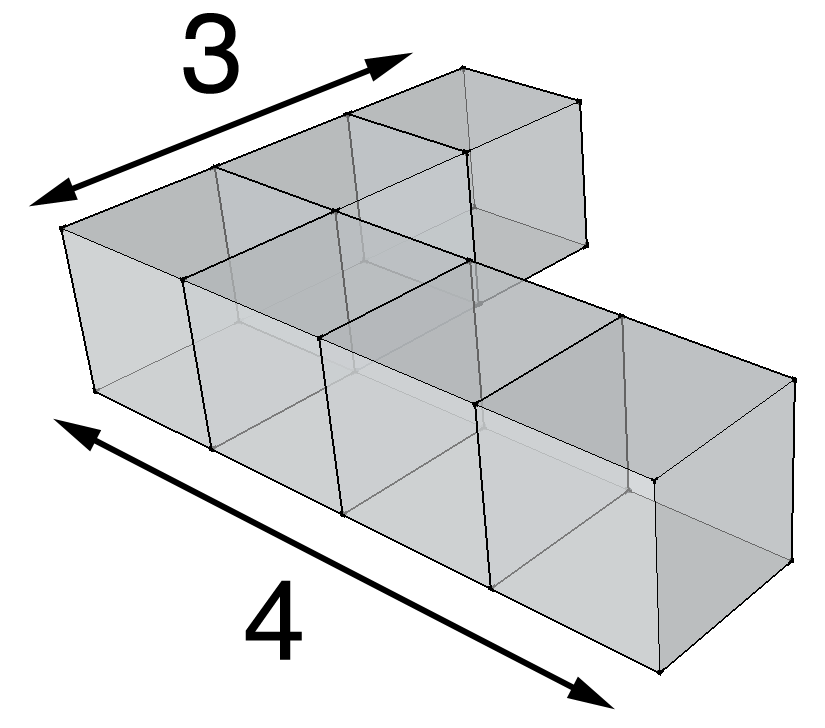
\includegraphics[width=0.9\textwidth]{./figures/3by4}
    \caption{A path with ratio $a:b = 3:4$}
		\label{fig:3by4}
  \end{minipage}
  \begin{minipage}[t]{.45\textwidth}
  \centering
  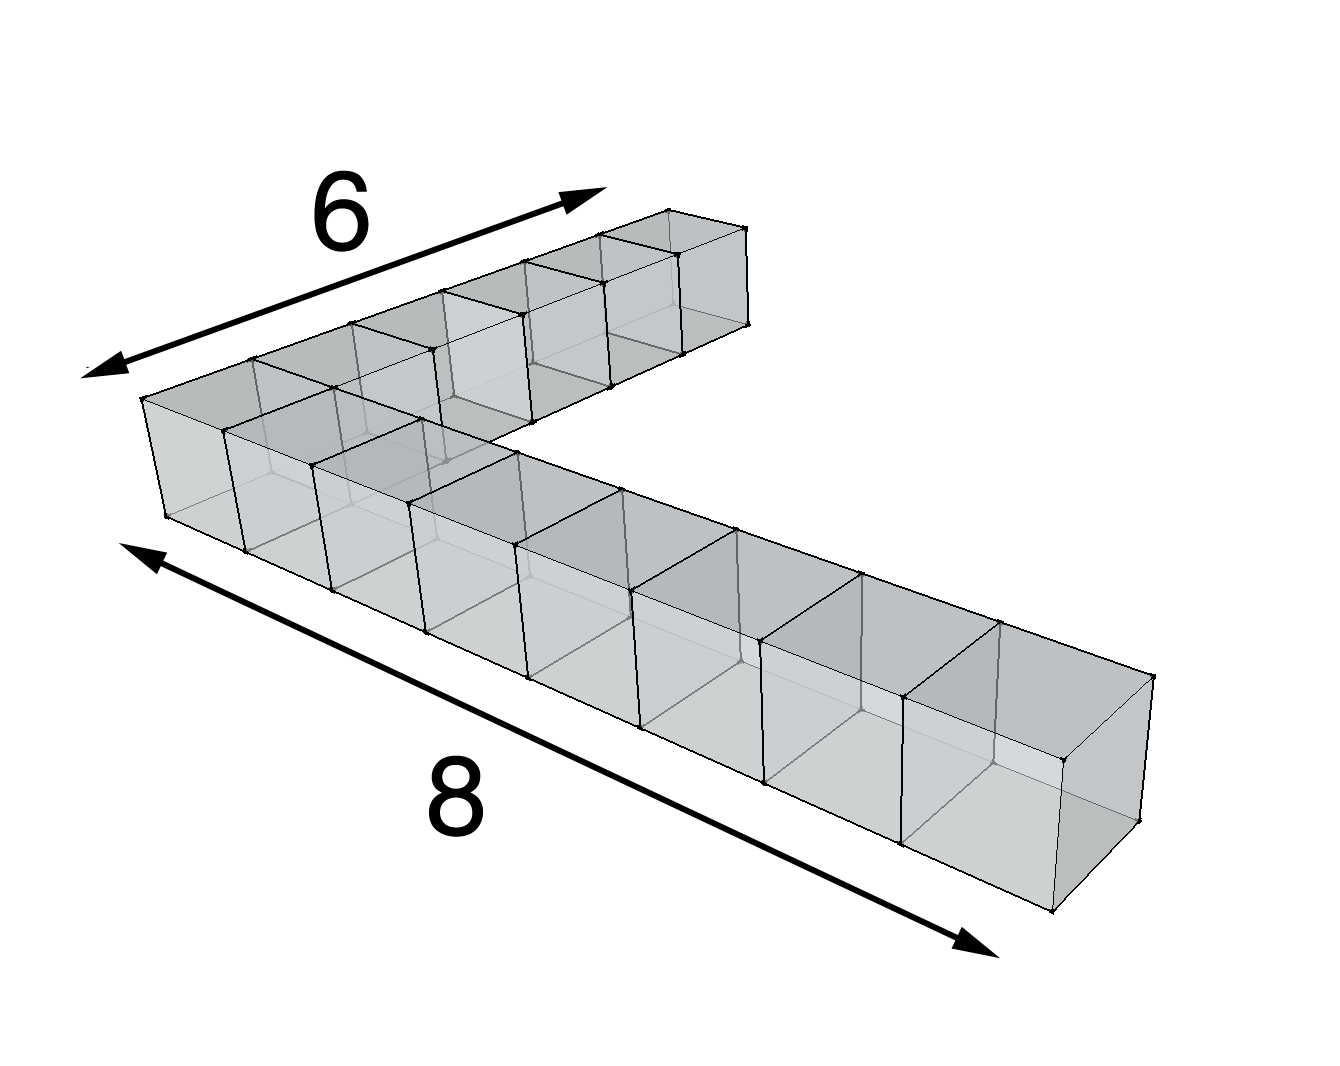
\includegraphics[width=0.9\textwidth]{./figures/6by8}
    \caption{Another path with ratio $a:b = 3:4$}
    \label{fig:6by8}
  \end{minipage}\hfill
  \begin{minipage}[t]{.45\textwidth}
  \centering
  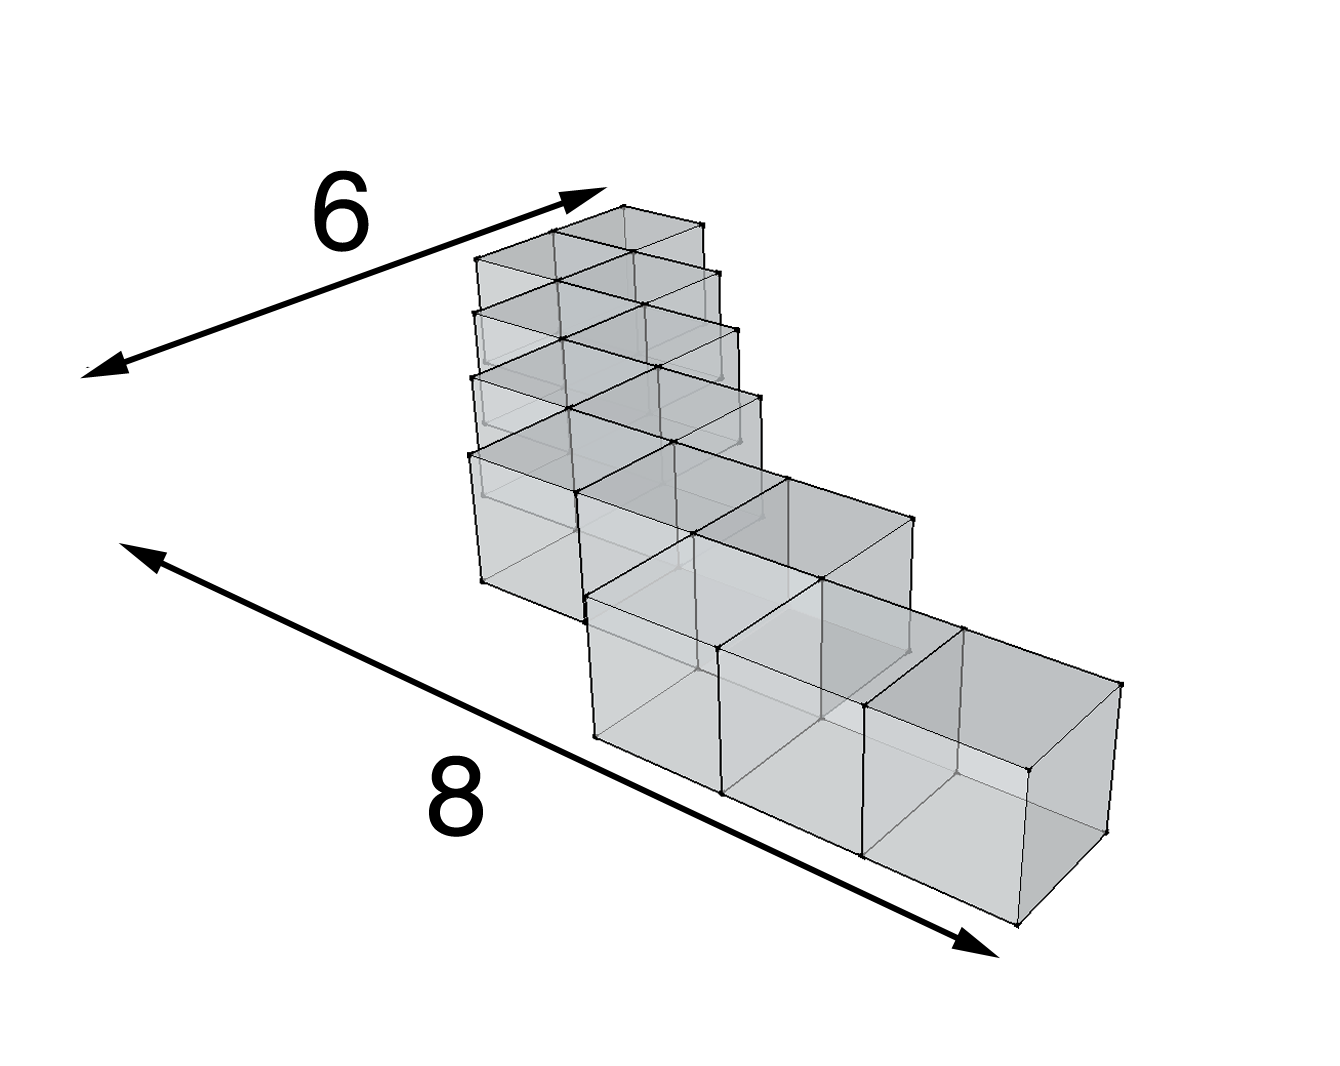
\includegraphics[width=0.9\textwidth]{./figures/6by8_squiggle}
    \caption{Alternate path also with ratio $a:b = 3:4$}
		\label{fig:6by8_squiggle}
  \end{minipage}
  \begin{minipage}[t]{.45\textwidth}
  \centering
  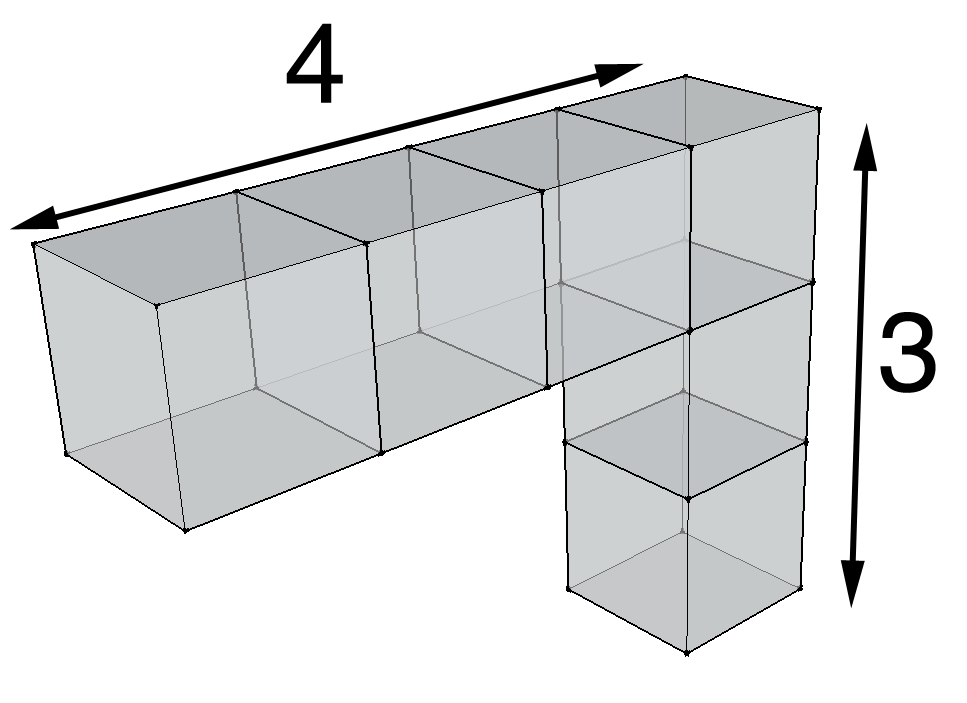
\includegraphics[width=0.9\textwidth]{./figures/3by4_upended.png}
  \caption{Cube with $a:b=3:4$ equivalent path after rotational transformation.}
  \label{fig:3by4_upended}
  \end{minipage}\hfill
\end{figure}

    

The ratio cube is fixed relative to the orientation of the axis, but there are 24 rotational symmetries for a cube.
Therefore given the ratio cubes for two paths $P_1$ and $P_2$, if path equivalence exists within some symmetry we can search this space and find, for example, other ratio equivalent paths as shown in Fig.~\ref{fig:3by4_upended}.



Method:
\begin{itemize}
 \item partition space into boxes
 \item enumerate the boxes
 \item map a concrete positional trace through space onto its uniquely corresponding boxes
 \item sync time frames of box-traces to infer spatio-temporal properties
 \item using the spatio-temporal box-trace, derive properties (given elsewhere)
\end{itemize}

\emph{Selecting appropriate box size}

Different box sizes may generate very different properties.

\emph{Too small of a box} If you choose the boxes to be relatively small, the trace may show a teleport, which we define as a spatially disconnected box-trace.
If there are gaps of disconnected boxes, and two entities collide in the unaccounted for space, the violation of box-independence will not be inferred.

\emph{Too big of a box} If you choose the boxes to be relatively large, this may be too rough of an over approximation.
For an extreme example, an entity never registers "leaving home" if its initial box is the size of the given dimensions.
Sometimes large over-approximations are desired, such as if you only want to examine the movements across two ``hemispheres" of an entity's space.
